\documentclass[10pt,a4paper]{article}
\usepackage[margin=2.1cm]{geometry}
\usepackage{amsmath,amssymb,amsthm,graphicx,booktabs,caption,float,xcolor,enumitem,array}
\usepackage{tikz}
\usetikzlibrary{arrows.meta,positioning}
\usepackage[colorlinks=true,linkcolor=blue!50!black,citecolor=blue!50!black,urlcolor=blue!50!black]{hyperref}
\captionsetup{font=small,labelfont=bf}
\setlist{itemsep=1pt,topsep=3pt}
\graphicspath{{figures/}}
\definecolor{cA}{HTML}{3b75af}
\definecolor{cC}{HTML}{d1495b}
\newtheorem{result}{Result}

\title{\textbf{The 15-agent campaign: reading reversal and persistence}\\[2pt]
\large in four setups, with the theory on the same grid}
\author{Claude (\nolinkurl{analysis/15_agent_simulation/})}
\date{Report, 30 October 2026 (runs of 29--30 October 2026)}

\begin{document}
\maketitle

\begin{abstract}
\noindent
\textbf{Design.} We reran Simulation 2 with 15 Bayesian agents in four setups: task003 and MuSR Object Placements (OP),
each in a \emph{symmetric} version (the agents' facts jointly prove the correct answer A0) and a new \emph{uniform
no-solution} version (the agents' facts, and the controller's single pool, each combine to about $(\tfrac13,\tfrac13,
\tfrac13)$). The grid has 8 reading levels $q$, 8 memory levels $\rho$ spaced evenly in memory lifetime, standard
against deduplicated reading, a false controller and its paired silent arm, run to $t=130$ with 1,000 paths per cell:
1,024 cells in all.

\textbf{Findings.}
\begin{itemize}
\item \textbf{The reading reversal appears in all four setups.} Reading more helps the controller at short memory and
  protects the swarm at long memory.
\item \textbf{One quantity sets where it happens:} the number of posts an agent reads during one memory lifetime,
  $q\tau$. At the crossover, $q\tau^*\approx 8$--$14$ in task003, 5--8 in OP symmetric and 13--23 in OP no-solution,
  nearly constant across a 16-fold range of $q$. The mean-field theory predicts this collapse and its cause, accumulated
  own evidence, but crosses about three times earlier ($q\tau^*\approx2.5$--$4$).
\item \textbf{Persistence:} task003 keeps nearly all its effect for 100 time units after the controller stops (median
  retention 0.93--1.0 at $q\ge4$); OP keeps less (0.82--0.83) and fades strongly at low $q$.
\item \textbf{Deduplicated reading is not a defence:} it raises the controller's effect by 24--36\% at short memory and
  lowers it only at long memory.
\end{itemize}
Of seven pre-registered predictions, four are met, and three fail (P2, P5, P6).
\end{abstract}

\tableofcontents
\clearpage

% ======================================================================================================================
\section{Design}
\label{sec:design}

\paragraph{The swarm and the controller.} $N=15$ exact Bayesian agents act at random times (rate 1).
\begin{itemize}
\item \textbf{Reading:} at each action an agent reads $q$ posts from the $W=30$ newest posts on a shared board,
  excluding its own posts.
\item \textbf{Memory:} each remembered fact is forgotten at rate $\gamma=-\ln\rho$.
\item \textbf{Voting:} probability matching (the agent votes A$k$ with probability $P(\mathrm{A}k\mid\text{memory})$).
\item \textbf{Posting:} a fact that supports its vote in context.
\item \textbf{Controller:} until $t=30$ it posts at rate 1 the fact from its pool that most raises the wrong answer
  A2, given 8 posts it samples ($q_c=8$, budget 30, vote gate 0.75, proof stop). Then it falls silent.
\end{itemize}
Every controlled episode is paired with a silent episode that uses the same random streams (Fig.~\ref{fig:timeline}).

\begin{figure}[h]
\centering
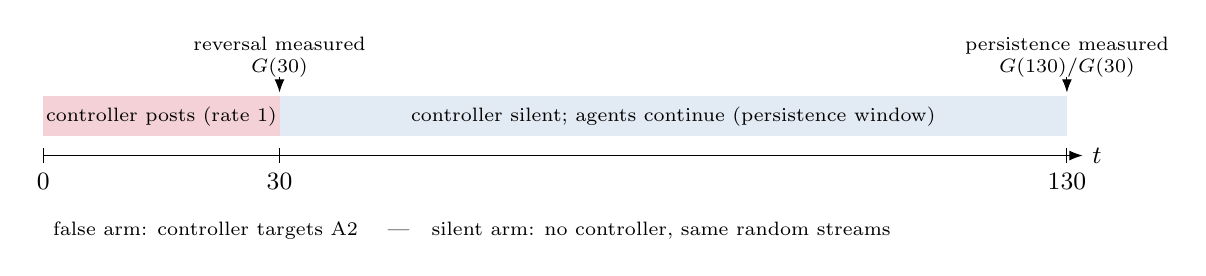
\begin{tikzpicture}[>=Latex, font=\small]
  \draw[->] (0,0) -- (13.2,0) node[right] {$t$};
  \foreach \x/\l in {0/0, 3/30, 13/130} {\draw (\x,0.1) -- (\x,-0.1) node[below] {\l};}
  \fill[cC!25] (0,0.25) rectangle (3,0.75);
  \node[font=\scriptsize] at (1.5,0.5) {controller posts (rate 1)};
  \fill[cA!15] (3,0.25) rectangle (13,0.75);
  \node[font=\scriptsize] at (8,0.5) {controller silent; agents continue (persistence window)};
  \node[font=\scriptsize, align=center] at (3,1.25) {reversal measured\\ $G(30)$};
  \draw[->] (3,1.0) -- (3,0.8);
  \node[font=\scriptsize, align=center] at (13,1.25) {persistence measured\\ $G(130)/G(30)$};
  \draw[->] (13,1.0) -- (13,0.8);
  \node[font=\scriptsize, align=left, anchor=west] at (0,-0.95) {false arm: controller targets A2 \quad|\quad
    silent arm: no controller, same random streams};
\end{tikzpicture}
\caption{\textbf{One paired episode.} The reversal is read at the controller's stop, persistence 100 time units later.}
\label{fig:timeline}
\end{figure}

\paragraph{The four setups} (\nolinkurl{analysis/15_agent_simulation/}; 15 agents, one distinct fact each).
\begin{itemize}
\item \textbf{Symmetric} (task003 and OP): the agents' facts jointly prove A0 and no fact or pair does. Separate A0
  and A2 controller pools, unchanged from the 24-agent setups.
\item \textbf{Uniform no-solution} (task003 and OP): the agents' facts combine to $(0.325, 0.350, 0.325)$ in task003
  and exactly $(\tfrac13,\tfrac13,\tfrac13)$ in OP. A single controller pool, also about uniform. Agents and pool
  together prove nothing.
\end{itemize}

\paragraph{Grid.} $q\in\{1,2,3,4,6,8,12,16\}$ and $\rho\in\{0.018, 0.135, 0.37, 0.61, 0.78, 0.88, 0.94, 1\}$. The
memory values are spaced evenly in the mean lifetime of a remembered fact,
\begin{equation}
\tau=-\frac{1}{\ln\rho}\ \in\ \{0.25, 0.5, 1, 2, 4, 8, 16, \infty\}.\label{eq:tau}
\end{equation}
Two reading modes:
\begin{itemize}
\item \textbf{standard:} $q$ posts;
\item \textbf{deduplicated:} $q$ distinct facts, each read through its newest copy.
\end{itemize}
The design and seven predictions were written down before the runs (\nolinkurl{00_preregistration.md}).

\paragraph{Measures.} For episode pair $e$ and time $t$, let $v^{\rm c}_e(t)$ and $v^{\rm s}_e(t)$ be the share of
A2 among the agents who have voted, in the controlled and silent arm. The controller's effect, its change with
reading, and its persistence are
\begin{align}
G(t)&=\frac{1}{n}\sum_{e=1}^{n}\big[v^{\rm c}_e(t)-v^{\rm s}_e(t)\big],\label{eq:G}\\
D(q_i\!\to\!q_{i+1})&=G(30;q_{i+1})-G(30;q_i),\label{eq:D}\\
\text{retention}&=G(130)/G(30)\quad(\text{reported where }G(30)>2\,\mathrm{se}).\label{eq:ret}
\end{align}
The \emph{crossover} $\tau^*$ for a reading step is the memory lifetime at which $D$ changes sign from positive to
negative, interpolated linearly in $\ln\tau$. Standard errors use the 1,000 episode pairs.

\paragraph{The theory on the same grid.} The mean-field fact-flow model of the closed theory work, at its P0 parameters
fixed on 27 October with $W=30$ and neutral reposting. Nothing is fitted to these runs. It gives the next-vote gap
$g(30)$, its reading increment, and its retention $g(130)/g(30)$ (\nolinkurl{analysis/theory_grid.py}).

% ======================================================================================================================
\section{Vote shares over time}
\label{sec:votes}
\begin{figure}[H]
\centering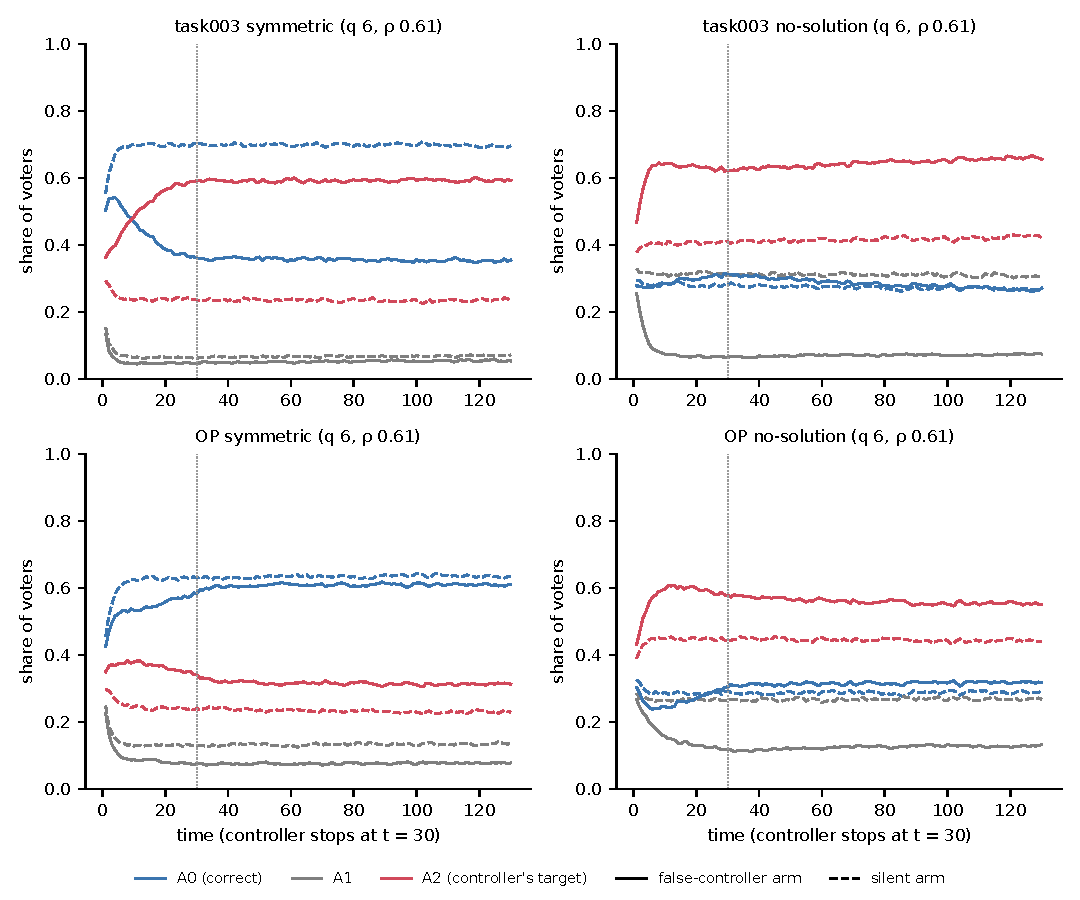
\includegraphics[width=0.92\linewidth]{fig01_vote_shares.pdf}
\caption{\textbf{Vote shares among voters} in the four setups at $q=6$, $\rho=0.61$ ($\tau=2$), standard reading.
Solid: false-controller arm; dashed: silent arm. The controller stops at $t=30$ (dotted line).}
\label{fig:votes}
\end{figure}
Figure~\ref{fig:votes} shows the raw data behind every later figure.
\begin{itemize}
\item \textbf{task003 symmetric.} The silent swarm settles at about 70\% for the correct A0. Under the false
  controller, A2 overtakes A0 by $t\approx8$ and reaches 60\%.
\item \textbf{OP symmetric.} The controller only slows the swarm's convergence on A0. Its lead in A2 is about 8
  points.
\item \textbf{No-solution setups.} Even the silent swarm leans to A2 (about 40--45\%), although its combined evidence
  is uniform. The controller adds 20 points in task003 and 13 in OP.
\item \textbf{After the stop,} the controlled arms barely move in task003. In OP no-solution, A2 drifts back slowly.
\end{itemize}

\begin{figure}[H]
\centering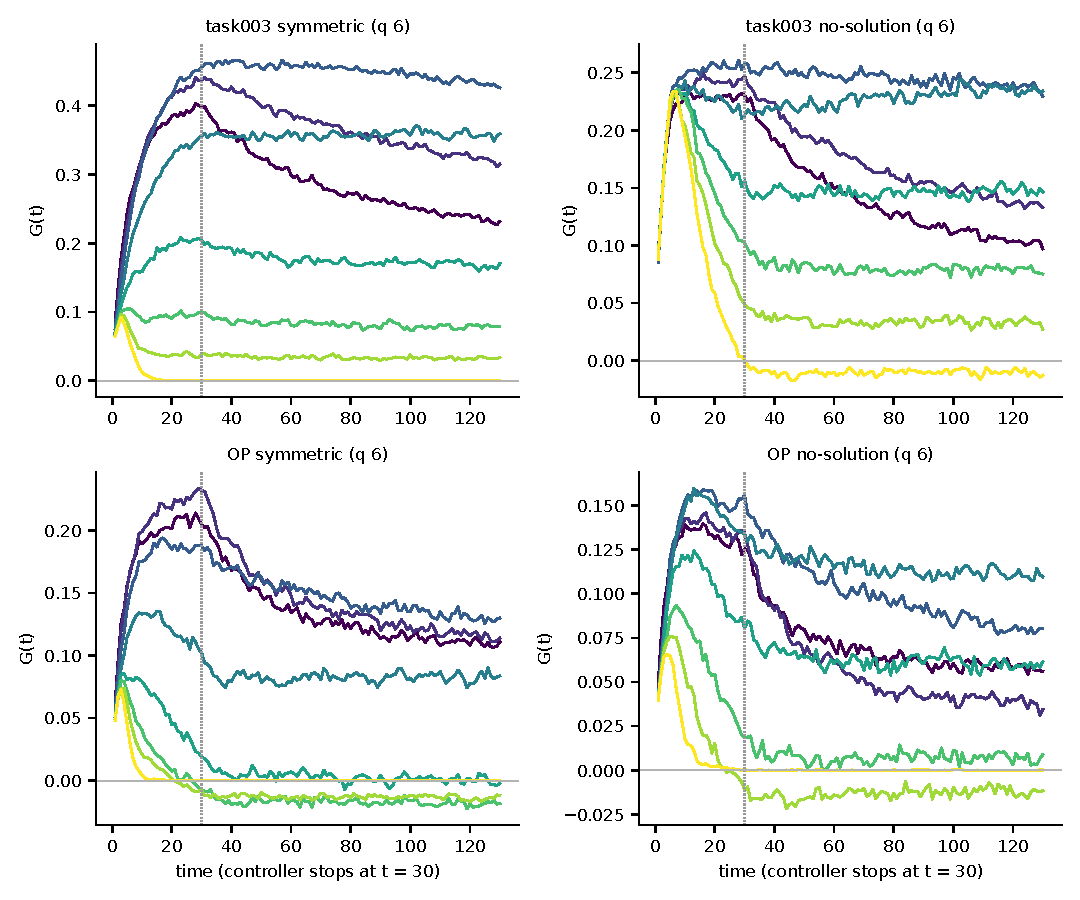
\includegraphics[width=0.92\linewidth]{fig02_gain_time.pdf}
\caption{\textbf{The controller's effect $G(t)$}, Eq.~\eqref{eq:G}, at $q=6$ for the eight memory levels (dark:
short memory; light: long memory).}
\label{fig:gaintime}
\end{figure}
Figure~\ref{fig:gaintime} shows the same effect across memory. $G$ rises during the attack, then stays, rises or decays
depending on memory. That is the subject of Section~\ref{sec:persistence}.

% ======================================================================================================================
\section{Pre-registered predictions}
\label{sec:prereg}
\begin{table}[H]
\centering\small
\caption{\textbf{The seven predictions}, evaluated exactly as pre-registered
(\nolinkurl{analysis/evaluate_predictions.py}; details in \nolinkurl{predictions.csv}).}
\label{tab:prereg}
\begin{tabular}{@{}p{0.39\linewidth}l p{0.41\linewidth}@{}}\toprule
prediction & verdict & evidence\\\midrule
P1 reversal in all four setups (some step among $1\to2$, \dots, $4\to6$) & \textbf{met} & all four steps reverse in
every setup\\
P2 crossover never moves to longer memory as $q$ grows (at most one violation per setup) & \textbf{failed} & task003:
0 violations; OP symmetric 2, OP no-solution 1 (all where $|D|<2\,$se)\\
P3 symmetric crosses at shorter memory than no-solution ($3\to4$, $4\to6$) & \textbf{met} & task003 2.84 vs 3.25 and
1.79 vs 1.84; OP 1.29 vs 3.71 and 1.13 vs 2.75\\
P4 task003 retains more than OP ($q=6$, $\rho$ 0.37--0.78), task003 $\ge0.7$ & \textbf{met} & task003 higher in 6 of
6; task003 0.83--1.10\\
P5 deduplication lowers $G$ in $\ge80\%$ of cells, by $\ge15\%$ & \textbf{failed} & lower in only 31\% (64 cells) or
42\% (48 cells); mean change $+11\%$ or $+4\%$\\
P6 deduplication does not cost silent accuracy ($>0.02$) & \textbf{failed} & holds in three setups; OP no-solution:
silent A2 share rises by more than 0.02 in 9 of 16 cells\\
P7 the reversal survives deduplication & \textbf{met} & all four setups\\\bottomrule
\end{tabular}
\end{table}
\textbf{A flaw in the pre-registration.} P5 says ``$\rho\le0.61$'' but counts ``3 $\rho$ values (48 cells)''. The grid
has four values up to 0.61. Both readings are reported, and the verdict is the same.

% ======================================================================================================================
\section{Reading reversal}
\label{sec:reversal}

\subsection{The phase diagrams}
\begin{figure}[H]
\centering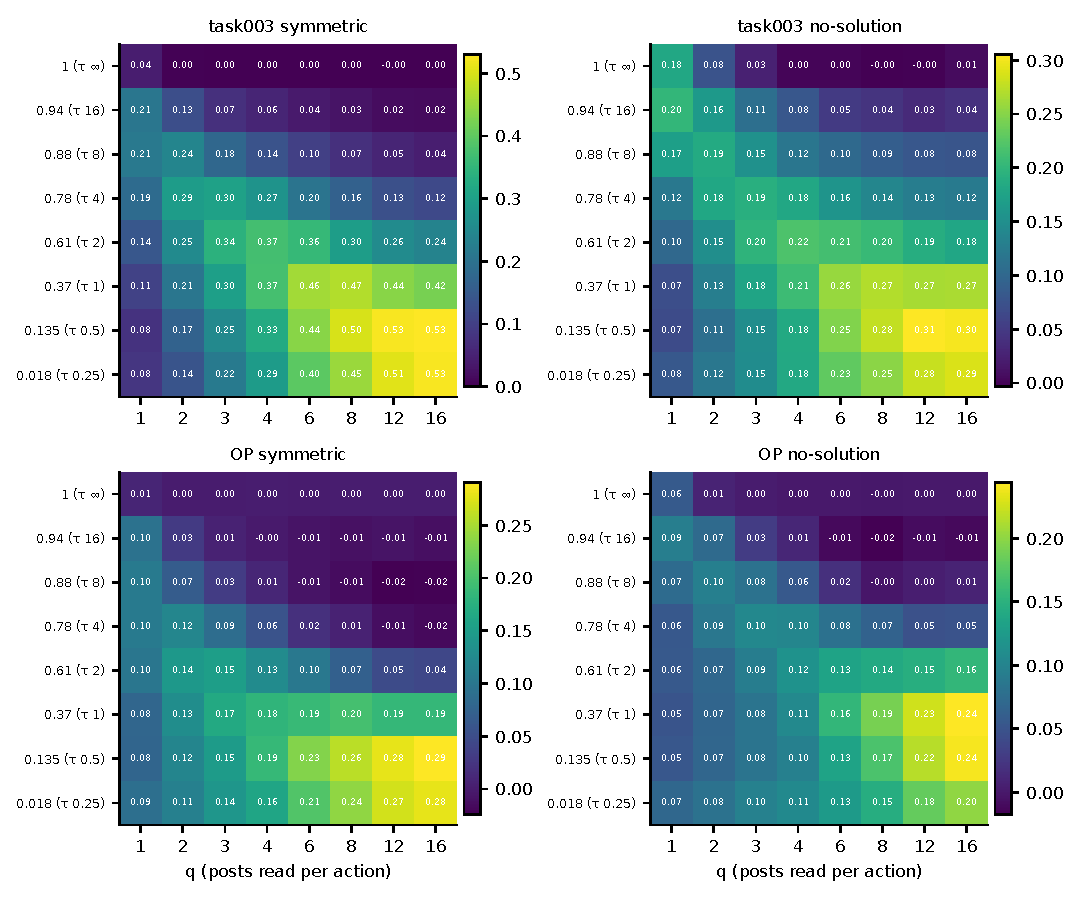
\includegraphics[width=0.9\linewidth]{fig03_gain_map.pdf}
\caption{\textbf{Phase diagram of the controller's effect} $G(30)$ over reading $q$ and memory $\rho$ (lifetime
$\tau$ in brackets), standard reading.}
\label{fig:gmap}
\end{figure}
\begin{figure}[H]
\centering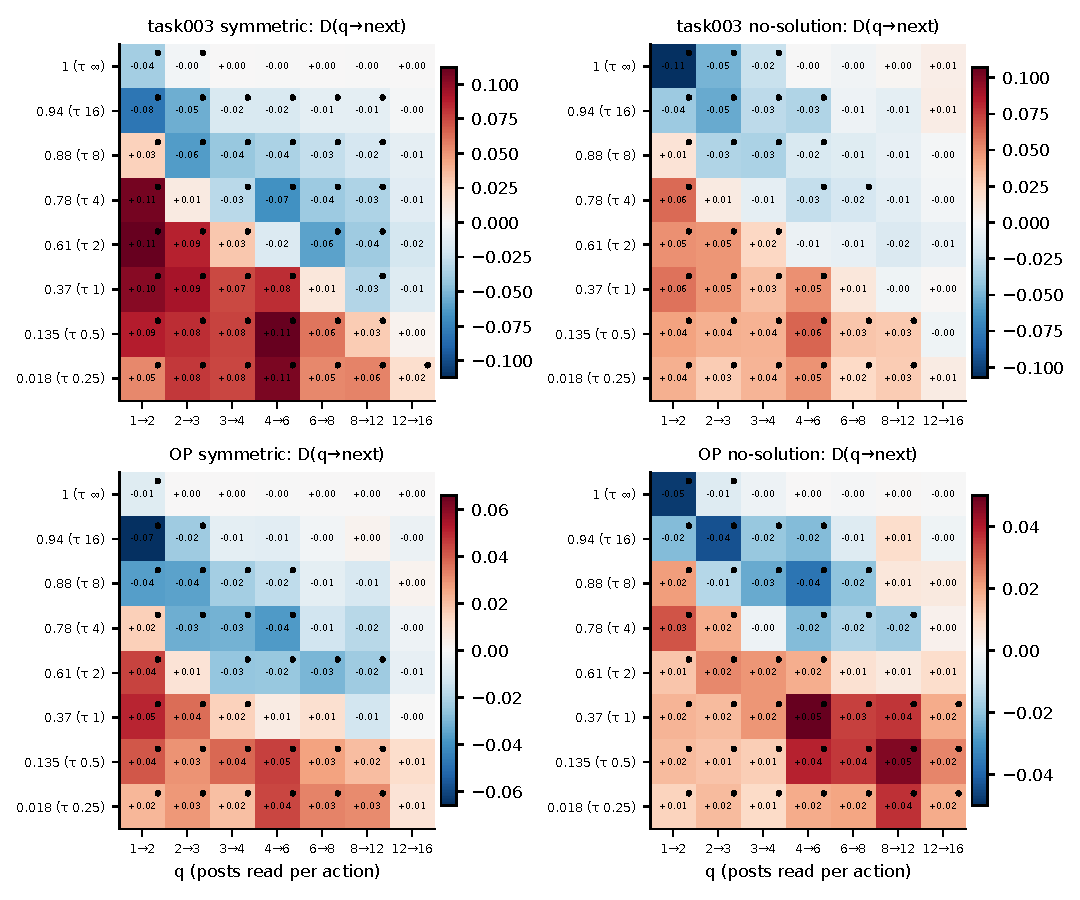
\includegraphics[width=0.9\linewidth]{fig04_increment_map.pdf}
\caption{\textbf{Phase diagram of the reading increment} $D(q\to\text{next } q)$, Eq.~\eqref{eq:D}. Red: reading more
helps the controller; blue: reading more protects the swarm. Dots: $|D|>2\,$se.}
\label{fig:dmap}
\end{figure}
\begin{result}[the reversal is universal across setups]
In every setup the $(q,\rho)$ plane splits into two regions along a diagonal (Fig.~\ref{fig:dmap}):
\begin{itemize}
\item \textbf{lower left (short memory, little reading):} reading more helps the controller ($D>0$);
\item \textbf{upper right (long memory, much reading):} reading more protects ($D<0$).
\end{itemize}
The largest effects are in task003 symmetric, where $G(30)$ reaches 0.53 at short memory and $q=16$
(Fig.~\ref{fig:gmap}). With perfect memory ($\rho=1$) and $q\ge3$, the symmetric swarms always reach the proof, and
$G=0$.
\end{result}

\subsection{One number sets the crossover: reads per memory lifetime}
\begin{figure}[H]
\centering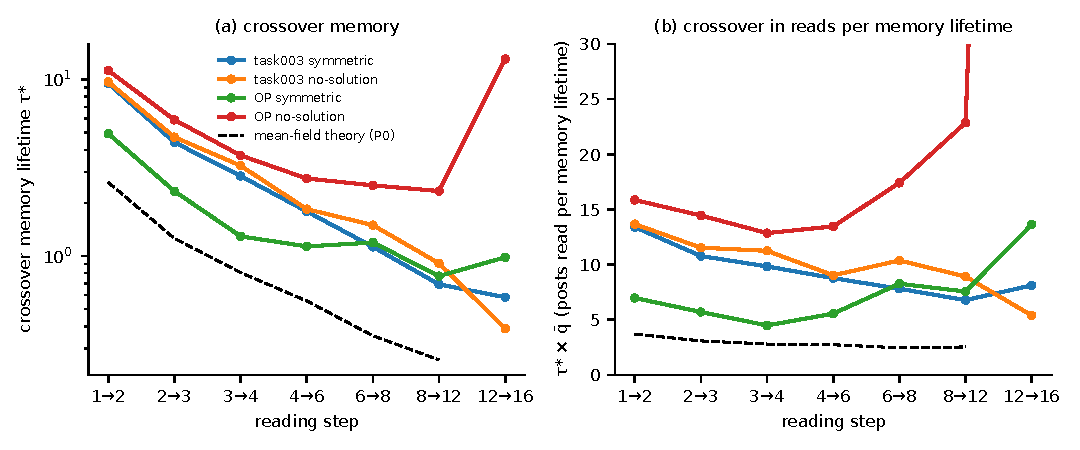
\includegraphics[width=0.95\linewidth]{fig05_crossovers.pdf}
\caption{\textbf{(a)} Crossover memory lifetime $\tau^*$ for each reading step. \textbf{(b)} The same, multiplied by
the step's geometric-mean reading level $\bar q$: posts read per memory lifetime at the crossover. Dashed: the
mean-field theory. The OP no-solution value at $12\to16$ (180, off the axis) comes from increments within noise.}
\label{fig:cross}
\end{figure}
Across a 16-fold range of $q$, $\tau^*$ falls roughly as $1/q$ (Fig.~\ref{fig:cross}a), so
\begin{equation}
q\,\tau^*\approx c_{\rm setup},\qquad c\approx 8\text{--}14\ (\text{task003}),\ 5\text{--}8\ (\text{OP symmetric}),\
13\text{--}23\ (\text{OP no-solution}),\label{eq:collapse}
\end{equation}
over the steps $1\to2$ to $8\to12$ (Fig.~\ref{fig:cross}b; Table~\ref{tab:cross}).
\begin{table}[H]
\centering\small
\caption{\textbf{Posts read per memory lifetime at the crossover}, $\bar q\,\tau^*$.}
\label{tab:cross}
\begin{tabular}{@{}lrrrrrrr@{}}\toprule
setup & $1\to2$ & $2\to3$ & $3\to4$ & $4\to6$ & $6\to8$ & $8\to12$ & $12\to16$\\\midrule
task003 symmetric & 13.4 & 10.8 & 9.8 & 8.8 & 7.8 & 6.8 & 8.1\\
task003 no-solution & 13.7 & 11.5 & 11.2 & 9.0 & 10.4 & 8.9 & 5.4\\
OP symmetric & 7.0 & 5.7 & 4.5 & 5.6 & 8.3 & 7.6 & 13.6\\
OP no-solution & 15.9 & 14.4 & 12.9 & 13.5 & 17.4 & 22.9 & (noise)\\
mean-field theory & 3.7 & 3.1 & 2.8 & 2.7 & 2.5 & 2.5 & --\\\bottomrule
\end{tabular}
\end{table}

\paragraph{Why the product $q\tau$: a derivation from the theory.} In the fact-flow model, an agent's chance of holding
a given own fact obeys $\dot m_A=(1-m_A)r_A-\gamma m_A$, with reading chance $r_A=1-(1-b_A/F_A)^q$. On a steady board
the holding chance settles at
\begin{equation}
m_A^*=\frac{r_A}{r_A+\gamma}\ \approx\ \frac{r_A}{\gamma}\ \approx\ \frac{q\,b_A}{F_A}\,\tau\qquad(r_A\ll\gamma,\ b_A\ll
F_A),\label{eq:mscaling}
\end{equation}
so the number of own facts held, $M_A=F_Am_A^*\approx b_A\,q\tau$, depends on $q$ and $\tau$ only through their
product. The reversal identity of the common theory,
\begin{equation}
\partial_q g=\underbrace{\sigma'(x_c)\,\partial_q\Delta x}_{\text{exposure}}+\underbrace{\beta_A\,\partial_qM_A^{S}\,
\big[\sigma'(x_s)-\sigma'(x_c)\big]}_{\text{sensitivity}},\label{eq:rev}
\end{equation}
turns negative once accumulated own evidence $M_A$ has pushed the population far enough from the tipping point. That
happens at a fixed $M_A$, hence at a fixed $q\tau$. Two consequences:
\begin{itemize}
\item \textbf{The collapse, Eq.~\eqref{eq:collapse}, is predicted.} The theory's own crossovers show it
  (Table~\ref{tab:cross}, last row).
\item \textbf{The constant's order follows the counter-evidence strength.} OP symmetric, whose agents' facts argue
  most strongly against A2 (measured $\beta_A=1.14$ in the 24-agent setups), crosses earliest; the no-solution setups cross latest. Their counter-evidence was weak or negative in the old 24-agent no-proof
  setups; it has not yet been measured for the new uniform ones.
\end{itemize}
The collapse breaks down at large $q$, where Eq.~\eqref{eq:mscaling} saturates ($m_A\to1$), and in OP no-solution,
whose crossover stops moving at $\tau^*\approx2.3$--$2.8$ for $q\ge4$.

\subsection{Comparison with the theory}
\begin{figure}[H]
\centering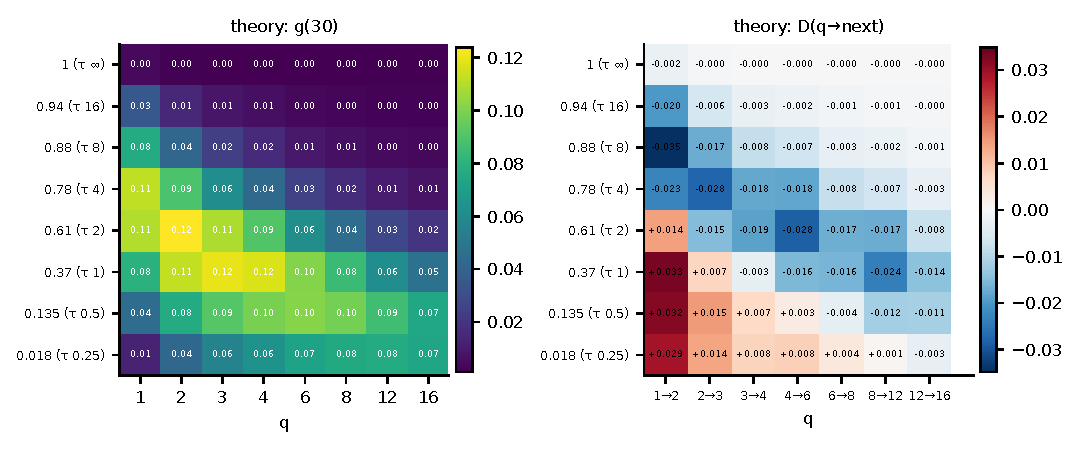
\includegraphics[width=0.95\linewidth]{fig06_theory_maps.pdf}
\caption{\textbf{The mean-field theory on the same grid} (P0, $W=30$, $\varepsilon=1$; nothing fitted): the next-vote
gap $g(30)$ and its reading increment.}
\label{fig:theory}
\end{figure}
Data (Fig.~\ref{fig:dmap}) and theory (Fig.~\ref{fig:theory}) are compared below.
\begin{itemize}
\item \textbf{Agreement:}
  \begin{itemize}
  \item the same two regions, separated by the same diagonal;
  \item the crossover moving to shorter memory as $q$ grows;
  \item the collapse in $q\tau$.
  \end{itemize}
\item \textbf{Disagreement:}
  \begin{itemize}
  \item the theory crosses about three times earlier ($c\approx2.5$--$4$ against 5--23);
  \item its effect is three to five times smaller ($g\le0.12$ against $G$ up to 0.53).
  \end{itemize}
  Both were expected from the finite-size analysis. The mean field has no extinction of the agents' sparse facts, so it
  overstates how quickly own evidence accumulates and understates the controller.
\end{itemize}

\paragraph{When the controller backfires.} In OP symmetric at long memory and large $q$, and in OP no-solution at
$\rho=0.94$, $G$ is significantly \emph{negative} (10 cells; largest $-0.024$, OP symmetric $q=12$, $\rho=0.88$). The
false controller there helps the swarm. Its A2 pool, combined with the agents' facts, proves A0, and long-memory agents
who read a lot assemble that proof.

\subsection{Deduplicated reading}
\begin{figure}[H]
\centering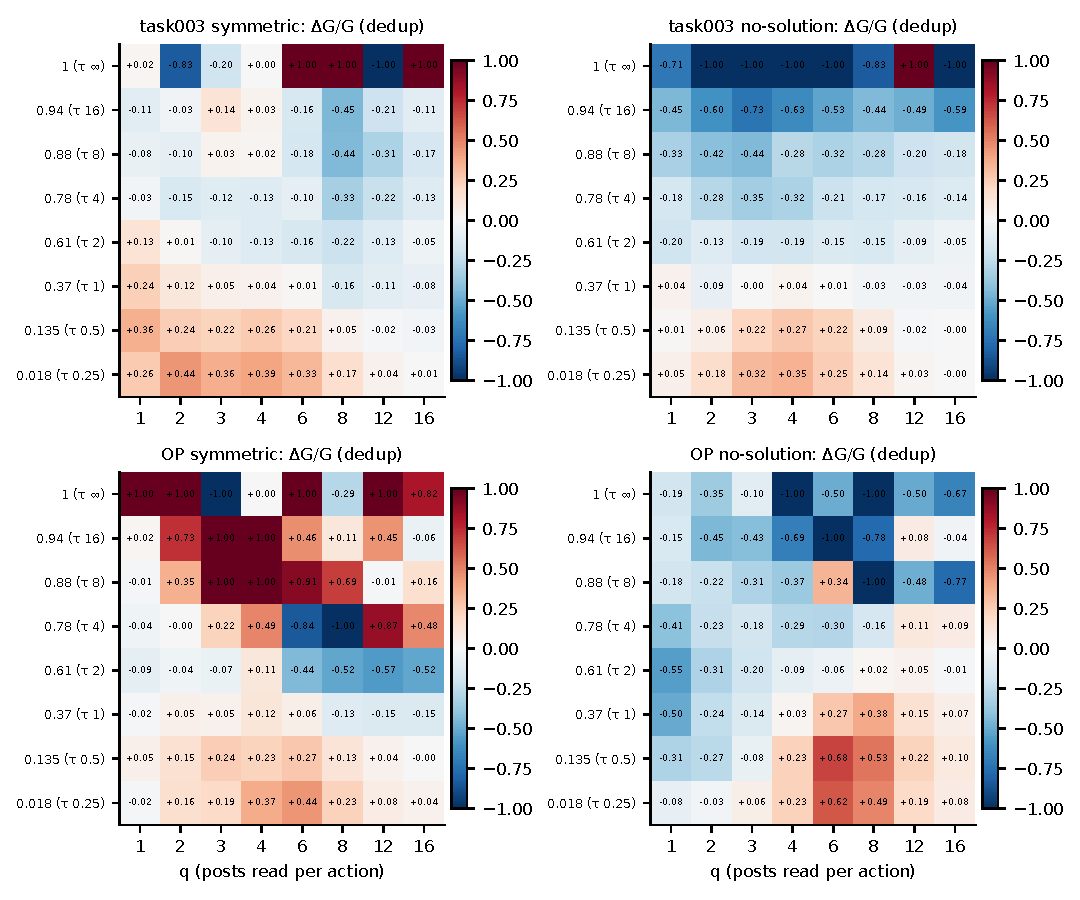
\includegraphics[width=0.9\linewidth]{fig07_dedup_map.pdf}
\caption{\textbf{Relative change of $G(30)$ under deduplicated reading}, $(G_{\rm dedup}-G)/G$ (clipped to $\pm1$).}
\label{fig:dedup}
\end{figure}
\begin{figure}[H]
\centering
\begin{minipage}{0.49\linewidth}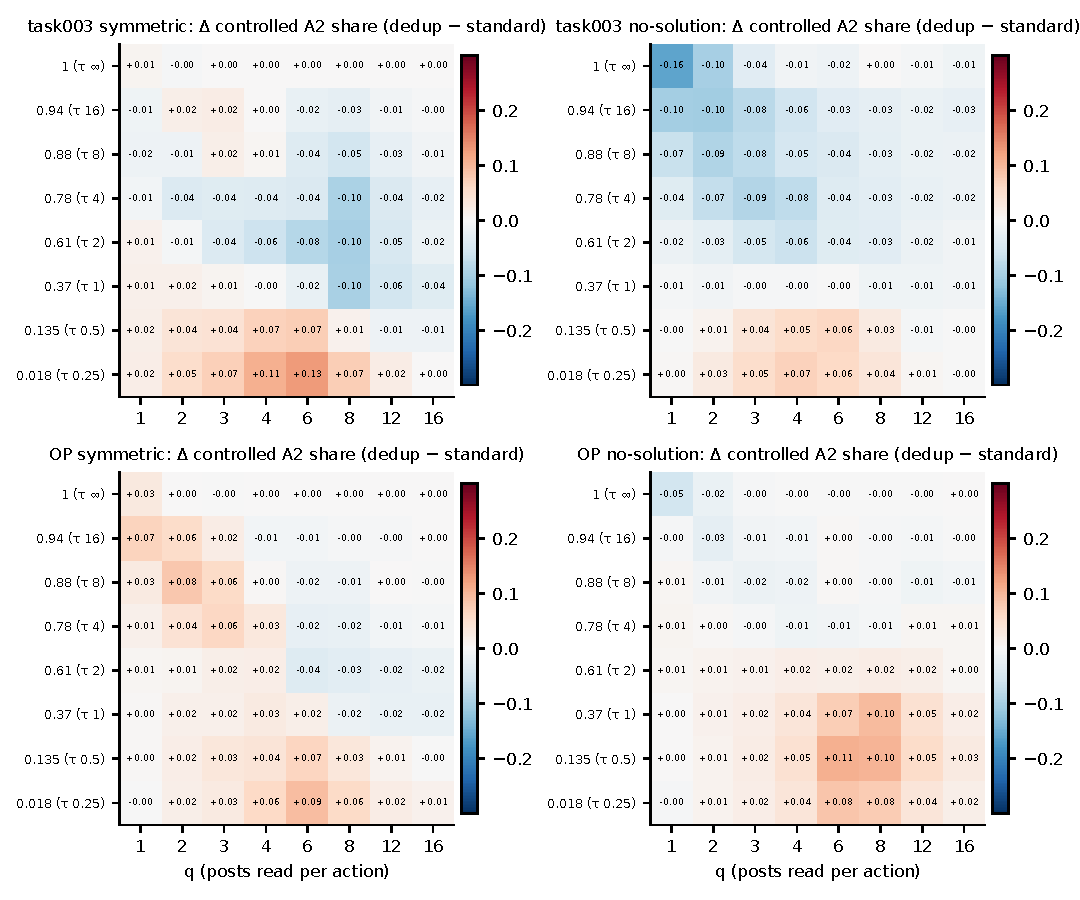
\includegraphics[width=\linewidth]{fig10_dedup_controlled_A2.pdf}\end{minipage}\hfill
\begin{minipage}{0.49\linewidth}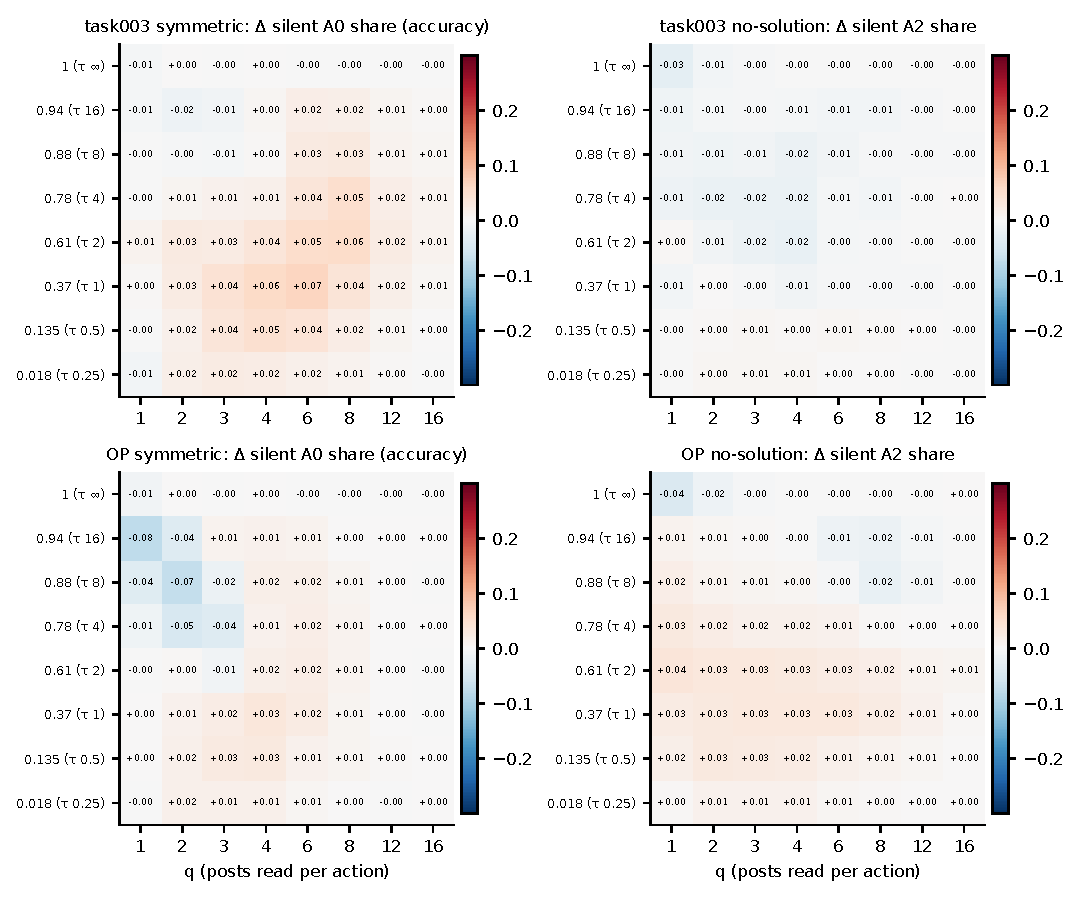
\includegraphics[width=\linewidth]{fig11_dedup_silent.pdf}\end{minipage}
\caption{\textbf{Absolute outcomes under deduplicated reading.} Left: change of the controlled arm's A2 share. Right:
change of the silent arm's accuracy (symmetric: A0 share) or A2 share (no-solution).}
\label{fig:dedupabs}
\end{figure}
\begin{result}[deduplicated reading is not a defence]
For $3\le q\le8$, the median relative change of $G$ under deduplication is:
\begin{itemize}
\item \textbf{short memory} ($\rho\le0.135$): $+24\%$ to $+36\%$ in every setup;
\item \textbf{middle memory:} $-11\%$ to $-1\%$;
\item \textbf{long memory} ($0.78$--$0.94$): $-12\%$ to $-34\%$, except OP symmetric, where $G$ is close to zero.
\end{itemize}
In absolute terms (Fig.~\ref{fig:dedupabs}):
\begin{itemize}
\item at short memory, the controlled arm's A2 share rises, for example from 0.72 to 0.85 in task003 symmetric at
  $\rho=0.018$, $q=6$;
\item the silent symmetric swarms become more accurate, for example A0 from 0.60 to 0.67 in task003 symmetric at
  $\rho=0.37$.
\end{itemize}
Deduplication makes agents read more distinct facts. That helps the unattacked swarm. In an attack, the controller's
distinct pool facts appear to benefit at least as much, most clearly at short memory.
\end{result}
\noindent This agrees with the ChatGPT agent's analytic result (blackboard \nolinkurl{2026-10-29_chatgpt_06}):
deduplication equalises the reading chance of every fact present, whoever posted it, so it removes copy advantage on
both sides. The 30-post window holds on average only 6--8 distinct facts (range 2--13, counted from the recorded posts), so
deduplicated reading saturates: under it, $G$ is flat for $q\ge8$ (\nolinkurl{table_gain_t30.csv}). Once $q$ exceeds
the number of distinct facts, reading more brings nothing new.

% ======================================================================================================================
\section{Persistence}
\label{sec:persistence}
\begin{figure}[H]
\centering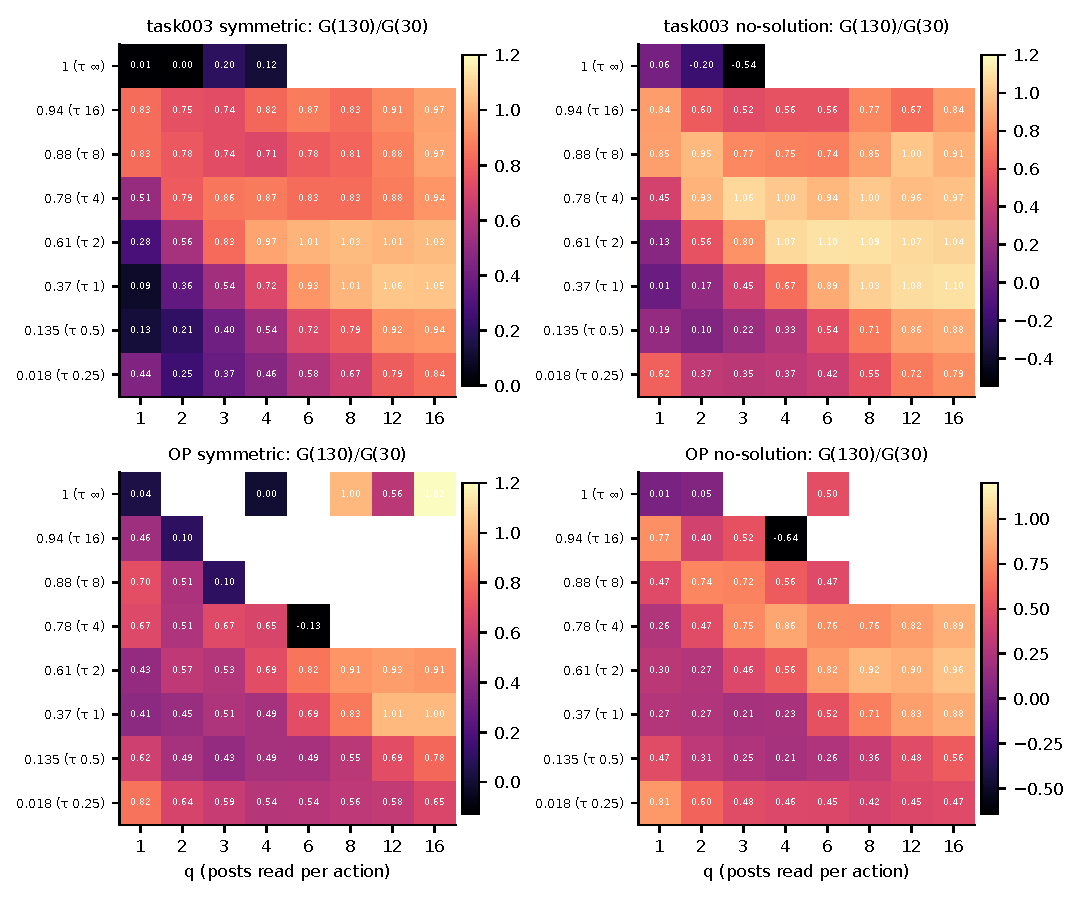
\includegraphics[width=0.9\linewidth]{fig08_retention_map.pdf}
\caption{\textbf{Phase diagram of persistence}: the share of the effect still present 100 time units after the stop,
Eq.~\eqref{eq:ret}. Blank: $G(30)<2\,$se. Values far outside $[0,1.2]$ come from cells with a small $G(30)$ and are
noisy.}
\label{fig:ret}
\end{figure}
\begin{figure}[H]
\centering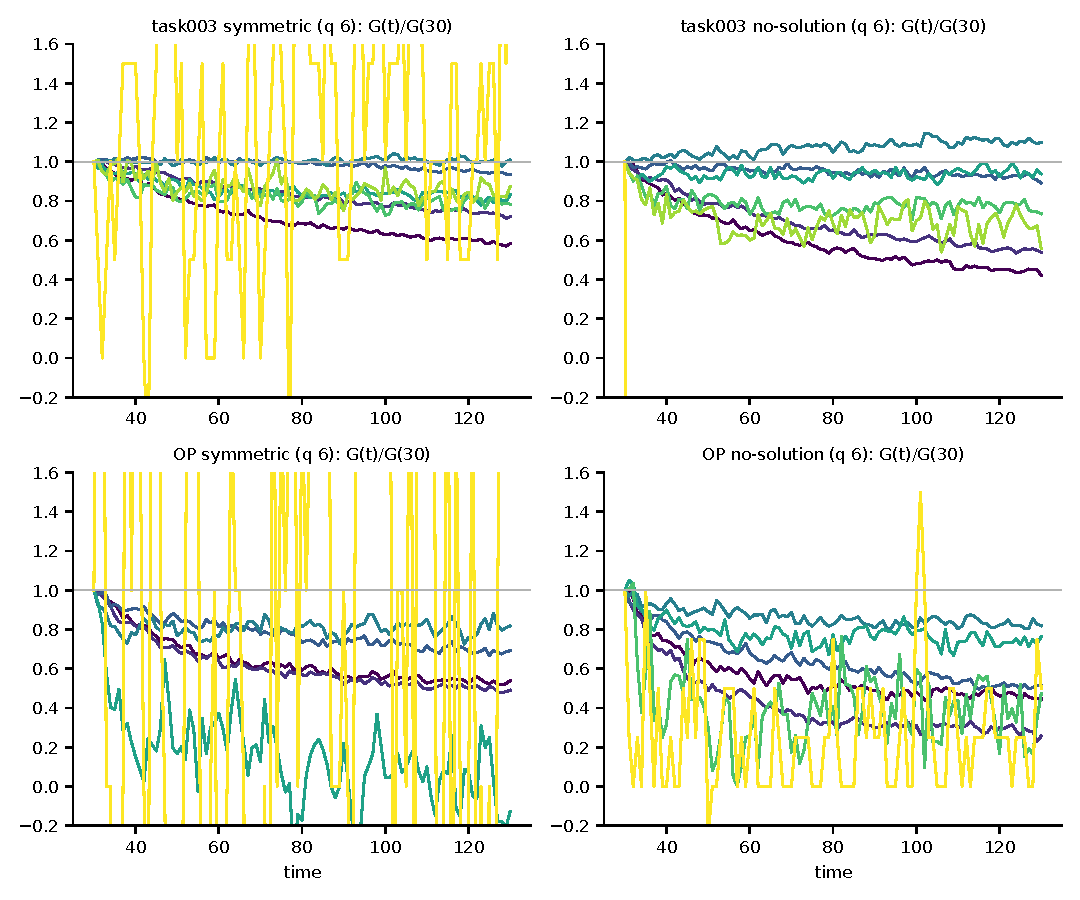
\includegraphics[width=0.9\linewidth]{fig09_gain_after_stop.pdf}
\caption{\textbf{$G(t)/G(30)$ after the stop} at $q=6$ for the eight memory levels.}
\label{fig:after}
\end{figure}
\begin{result}[persistence grows with reading and is stronger in task003]
\begin{itemize}
\item \textbf{Reading sustains it.} In every setup, retention rises with $q$ (Fig.~\ref{fig:ret}). At $q\le2$ and
  short memory the effect largely fades (median retention 0.18--0.55). At $q\ge4$ and $\rho$ 0.37--0.88 it is
  largely kept.
\item \textbf{The task contrast of the 24-agent runs reappears.} Median retention in that region is 0.93 (task003
  symmetric) and 1.00 (task003 no-solution), against 0.83 and 0.82 in OP. Retention above 1 in task003 means the
  effect keeps growing after the stop.
\item \textbf{OP fades most at short memory and little reading} (Fig.~\ref{fig:after}).
\end{itemize}
\end{result}

\paragraph{Comparison with the theory.} The theory explains persistence by a growth threshold for controller facts,
\begin{equation}
\mathcal R_C=\frac{q\,\kappa_C\,g_C}{\gamma\,H_{\rm post}}>1,\label{eq:RC}
\end{equation}
under which a copy of a controller fact makes more than one copy before it is lost. Since $\mathcal R_C\propto q\tau$,
the theory also predicts retention rising with reading and memory.
\begin{figure}[H]
\centering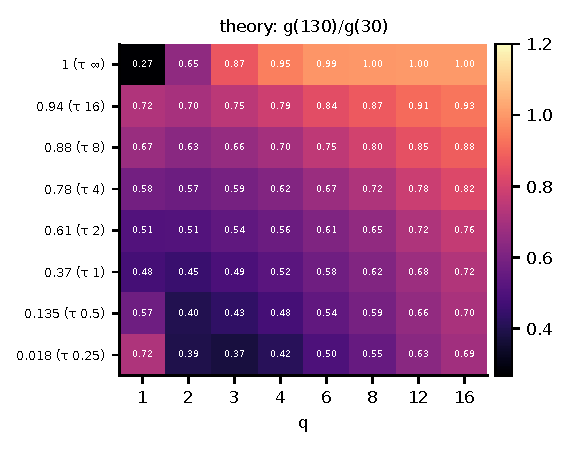
\includegraphics[width=0.42\linewidth]{fig12_theory_retention.pdf}
\caption{\textbf{The theory's retention} $g(130)/g(30)$ on the same grid.}
\label{fig:thret}
\end{figure}
\begin{itemize}
\item \textbf{Agreement:} the theory's retention (Fig.~\ref{fig:thret}) rises with $q$, from about 0.4 at $q=2$ to
  0.7--0.9 at $q=16$, as in the data.
\item \textbf{What it cannot show:} the task contrast. The model has no task structure. The common theory's candidate
  for the contrast is selection among circulating controller facts: OP's controller facts push toward A2 in fewer
  contexts, and support-based reposting then recirculates their least persuasive versions. That mechanism was found
  after seeing the data; this campaign does not test it.
\end{itemize}

% ======================================================================================================================
\section{Summary and next steps}
\begin{enumerate}
\item \textbf{Reading reversal.}
  \begin{itemize}
  \item It holds in all four setups (P1, P7).
  \item Its location is set by the number of posts read per memory lifetime, $q\tau^*\approx c$
    (Eq.~\ref{eq:collapse}). This is predicted by the theory through accumulated own evidence (Eq.~\ref{eq:mscaling}),
    though the theory's constant is about three times smaller.
  \item Stronger counter-evidence gives an earlier crossover (P3).
  \item P2 failed only through increments within noise in OP.
  \end{itemize}
\item \textbf{Persistence} rises with reading in every setup, as the threshold Eq.~\eqref{eq:RC} implies, and is
  stronger in task003 than in OP (P4).
\item \textbf{Deduplicated reading} raises the controller's effect at short memory and lowers it only at long memory
  (P5 failed). It improves the unattacked symmetric swarm. It is not a defence.
\item \textbf{Next:}
  \begin{itemize}
  \item a finite-size theory of the constant $c$ (why 8--14 rather than 2.5--4);
  \item a direct test of the selection mechanism for OP's weaker persistence, using the recorded posts;
  \item source refresh (the ChatGPT agent's proposal) as the next candidate defence;
  \item choosing cells for the 100-path LLM runs around the crossover diagonal.
  \end{itemize}
\end{enumerate}

\paragraph{Reproducibility.}
\begin{itemize}
\item Runs: \nolinkurl{results/2026-10-29_sim2_15agents_task003} and \nolinkurl{_op} (gitignored), configs in
  \nolinkurl{configs/}.
\item Pipeline: \nolinkurl{analysis/aggregate.py}, \nolinkurl{theory_grid.py}, \nolinkurl{figures.py},
  \nolinkurl{evaluate_predictions.py}.
\item Tables: \nolinkurl{table_gain_t30.csv}, \nolinkurl{table_crossovers.csv}, \nolinkurl{table_absolute_t30.csv} and
  \nolinkurl{predictions.csv}, in this folder.
\end{itemize}

\end{document}
